\documentclass[conference]{IEEEtran}
\pagestyle{plain}
%\IEEEoverridecommandlockouts
% The preceding line is only needed to identify funding in the first footnote. If that is unneeded, please comment it out.
% Template version as of 6/27/2024

\usepackage{cite}
\usepackage[ngerman]{babel}
\usepackage{amsmath,amssymb,amsfonts}
\usepackage{algorithmic}
\usepackage{graphicx}
\usepackage{textcomp}
\usepackage{listings}
\usepackage[utf8]{inputenc}
\usepackage[justification=centering]{caption} % Paket für Captions
\usepackage{xcolor}
\usepackage{url}
\def\BibTeX{{\rm B\kern-.05em{\sc i\kern-.025em b}\kern-.08em
    T\kern-.1667em\lower.7ex\hbox{E}\kern-.125emX}}
\begin{document}

\lstset{
    basicstyle=\normalfont\footnotesize,
    keywordstyle=\bfseries, % Nur fett, keine Farbe
    stringstyle=\color{violet},
    commentstyle=\color{green!70!black},
    showstringspaces=false,
    numbers=none,
    breaklines=true,
    captionpos=b,
}

\title{FPGAs in DBMS
}

\author{\IEEEauthorblockN{1\textsuperscript{st} Felix Grenzing}
    \IEEEauthorblockA{\textit{Universität Hamburg} \\
        Hamburg, Deutschland\\
        felix.grenzing@studium.uni-hamburg.de}
}

\maketitle

\begin{abstract}
    In diesem Paper werden verschiedene Ansätze zur Nutzung von FPGAs (Field Programmable Gate Arrays) in Datenbanksystemen untersucht.
    Es wird gezeigt, wie FPGAs als Beschleuniger für Datenbankoperationen eingesetzt werden können, um die Performance zu verbessern.
    Verschiedene Architekturen und Algorithmen, wie BitWeaving, IBEX, Caribou, DoppioDB und REGEXP\_LIKE, werden vorgestellt.
    Die Ergebnisse zeigen, dass FPGAs signifikante Leistungssteigerungen bieten können, insbesondere durch
    die Nutzung von Parallelität und hybriden Ansätzen. Herausforderungen wie begrenzte Ressourcen und die Komplexität der Entwicklung
    werden ebenfalls thematisiert. Abschließend wird ein Ausblick auf zukünftige Entwicklungen gegeben.
\end{abstract}

\begin{IEEEkeywords}
    FPGAs, DBMS, Hardware Acceleration
\end{IEEEkeywords}

\section{Einführung}
Datenbanken sind allgegenwärtig und werden universell vervendet. Von kleinen In-Memory Datenbanken, die in Embedded-Systemen laufen, bis
hin zu großen verteilten Datenbanksystemen, die in der Cloud betrieben werden. Große Datenbanksysteme müssen eine hohe Anzahl von Anfragen
mit hohem Durchsatz verarbeiten, was eine Herausforderung für die Hardware darstellt. CPUs sind die naheliegende Wahl für die Verarbeitung
von Datenbankanfragen, da sie flexibel, leistungsstark und allgegenwärtig sind. Besonders durch die Stagnation der CPU Leistung in den letzten Jahren
und der Evolution von Datenbankworkloads, kommen jedoch auch andere Hardwareeinheiten wie FPGAs als Beschleuniger in Betracht. Exemplarisch
werden in diesem Paper, basierend auf~\cite{lisa_column_2018} und~\cite{istvan_glass_2019} verschiedene Ansätze vorgestellt, wie FPGAs in Datenbanksystemen
eingesetzt werden können und welche Herausforderungen
sich ergeben. Die vorgestellten Ansätze sind BitWeaving, IBEX, Caribou, DoppioDB und das REGEXP\_LIKE Projekt~\cite{lisa_column_2018}~\cite{istvan_glass_2019}~\cite{li_bitweaving_2013}.

In~\ref{sec:begriffe} werden zunächst einige Begriffe erläutert. In~\ref{sec:einordnung} werden Pessimismus und Optimismus aus~\cite{istvan_glass_2019} gegenüber gestellt.
In~\ref{sec:col_scan_acc} wird die Column Scan Acceleration aus~\cite{lisa_column_2018} vorgestellt und die Erkenntnisse daraus zusammengefasst. In~\ref{sec:andere_ansätze}
werden weiter Beispiele für FPGA Beschleuniger aus~\cite{istvan_glass_2019} genannt. In~\ref{sec:road_ahead} wird eine Überschrift aus~\cite{istvan_glass_2019} in welchem die Zukunft thematisiert ist
aufgegriffen.
In~\ref{sec:fazit} werden die Erkenntnisse zusammengefasst und ein Ausblick gegeben.


\section{Begriffe} \label{sec:begriffe}
In~\cite{lisa_column_2018} und~\cite{istvan_glass_2019} werden verschidene Begriffe verwendet, die Erklärung bedürfen und in diesem Abschnitt
erläutert werden.


\subsection{FPGAs}
Ein FPGA (Field Programmable Gate Array) ist ein programmierbarer Schaltkreis, der aus einer Matrix von Logikblöcken besteht, die durch programmierbare Verbindungen miteinander verbunden sind.
Die Logikblöcke können durch den Nutzer programmiert werden, um beliebige logische Funktionen zu implementieren. Die Verbindungen zwischen den Logikblöcken können ebenfalls
programmiert werden, um die Logikblöcke miteinander zu verbinden. FPGAs sind flexibel und können für eine Vielzahl von Anwendungen eingesetzt werden, die von der Signalverarbeitung
über die Kryptographie bis hin zur Datenbankbeschleunigung reichen. FPGAs sind jedoch nicht so flexibel wie CPUs, da sie nur eine begrenzte Anzahl von Logikblöcken und Verbindungen
haben. FPGAs können stattdessen spezialisierte Algorithmen sehr effizient zu implementieren, da sie in der Lage sind, die Algorithmen in Hardware zu implementieren, was zu
einer hohen Parallelität und Geschwindigkeit führen kann. FPGAs werden auch häufig als Prototypen für ASICs (Application Specific Integrated Circuits) verwendet.

\subsection{Einsatzmöglichkeiten}

FPGAs können in Datenbanksystemen auf verschiedene Weisen eingesetzt werden und werden daher häufig auf diese Art kategorisiert. Die Einordnung basiert hierbei auf Position des Beschleunigers
in Bezug auf die Daten und die CPU\@.


Klassischer Weise gibt es On-the-Side Beschleuniger (Abbildung~\ref{fig:deployment}), wobei die CPU die Daten
verwaltet und der FPGA über eine Schnittstelle wie PCIe angebunden ist. Die CPU muss bei dieser Einsatzoption die Daten an den FPGA senden und die Ergebnisse wieder
empfangen. Diese Architektur wurde häufig auch mit GPUs umgesetzt.

Eine andere Möglichkeit ist die In Datapath Beschleunigung (Abbildung~\ref{fig:deployment}), bei der der FPGA direkt in den Datenpfad eingebunden ist. Der FPGA kann die Daten in Echtzeit
verarbeiten und die Ergebnisse mit gleicher Geschwindigkeit an die CPU zurückgeben. Häufig ist das Ziel die Datenmenge zu reduzieren, da nahe der
Datenquelle häufig höhere Bandbreiten zur Verfügung stehen. Die Architektur ist somit mit Smart-Storage Lösungen verwandt.

Eine dritte Möglichkeit ist die Koprozessor Architektur (Abbildung~\ref{fig:deployment}), bei der der FPGA als Koprozessor der CPU fungiert. Der FPGA ist auf demselben Chip wie die CPU
und hat häufig auch direkten Speicherzugriff. Flaschenhälse durch langsame Schnittstellen können so vermieden werden, was Vorteile gegenüber
\mbox{On-the-Side} Beschleunigern bieten kann.

\begin{figure*}[] % "b" sorgt dafür, dass das Bild unten auf der Seite platziert wird
    \centering
    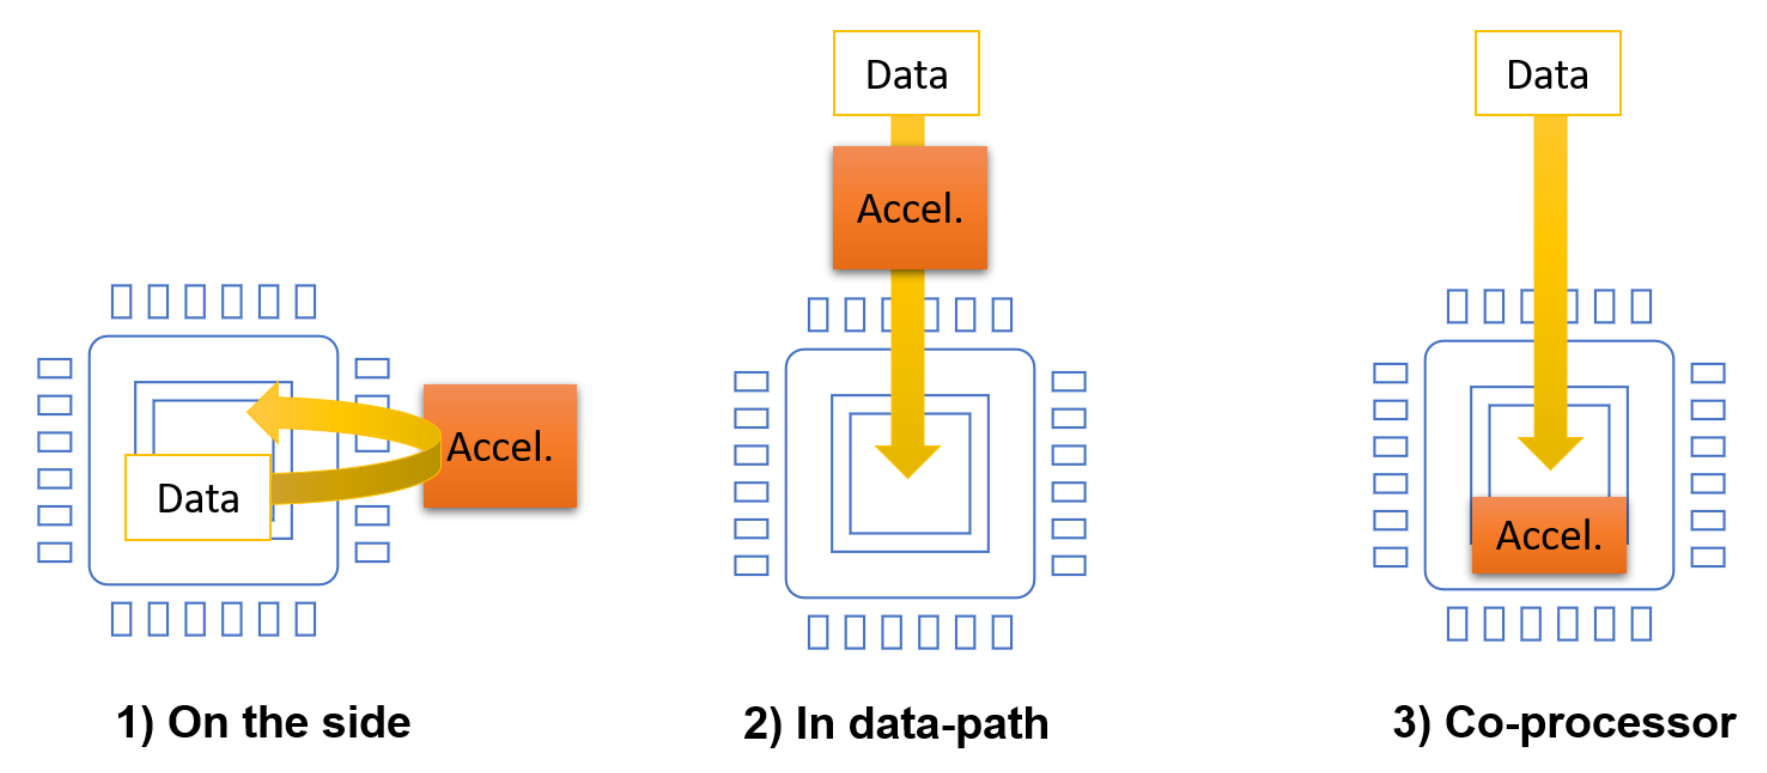
\includegraphics[width=0.85\textwidth]{imgs/deployment.png}
    \caption{Einsatzmöglichkeiten von FPGAs in Datenbanksystemen~\cite{istvan_glass_2019}}
    \label{fig:deployment}
\end{figure*}




% \begin{figure}[htbp]
%     \centering
%     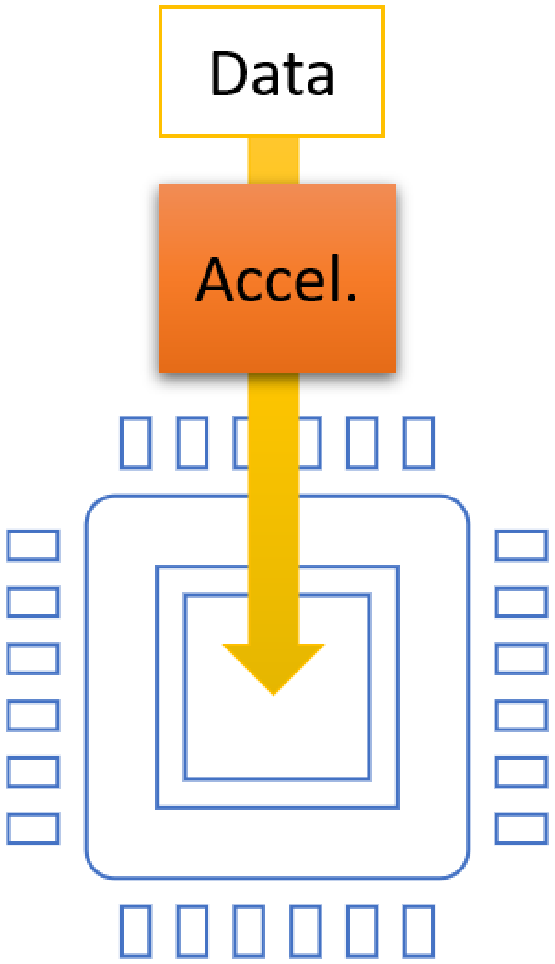
\includegraphics[width=0.1\textwidth]{imgs/InDatapath.png}
%     \caption{In Datapath Architektur}
%     \label{fig:indatapath}
% \end{figure}

% \begin{figure}[htbp]
%     \centering
%     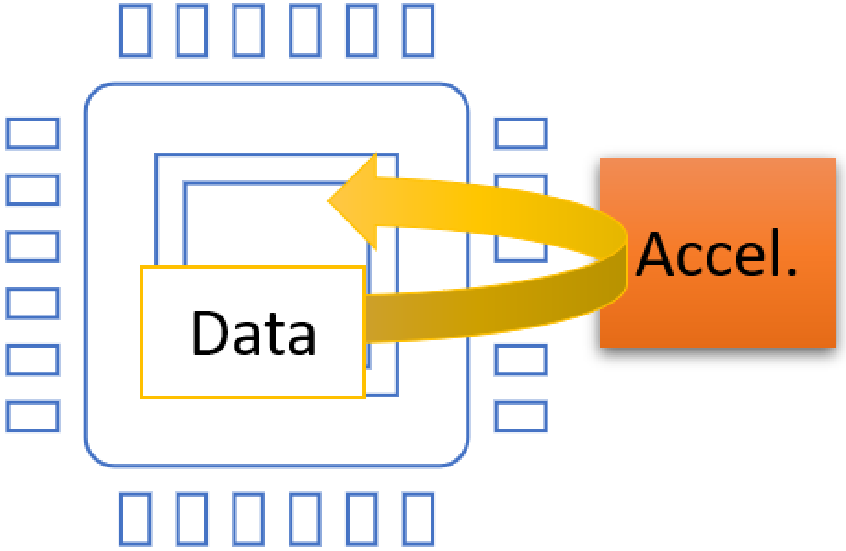
\includegraphics[width=0.15\textwidth]{imgs/OnTheSide.png}
%     \caption{On The Side Architektur}
%     \label{fig:ontheside}
% \end{figure}


% \begin{figure}[htbp]
%     \centering
%     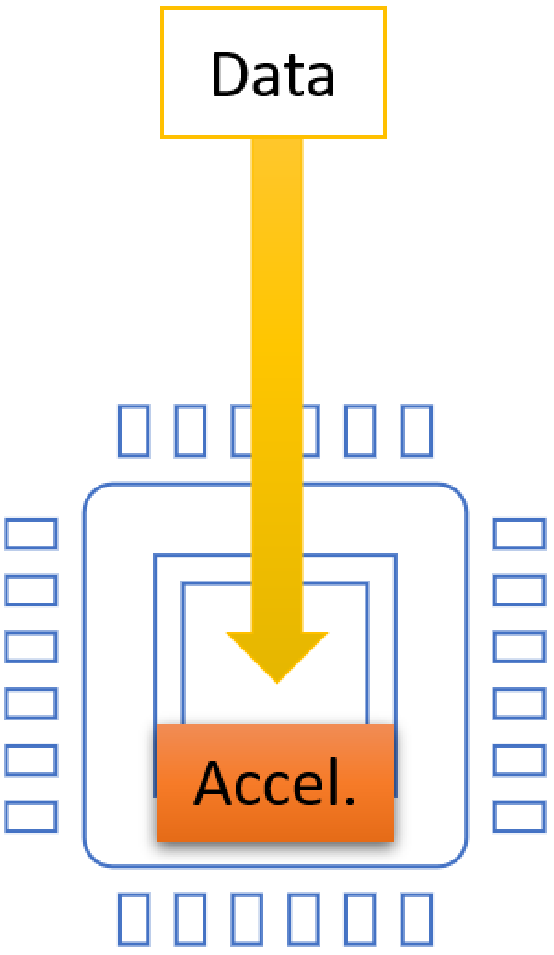
\includegraphics[width=0.1\textwidth]{imgs/Coprocessor.png}
%     \caption{Koprozessor Architektur}
%     \label{fig:coprocessor}
% \end{figure}

\subsection{Pipelining und Datenparallelität}
Zwei wichtige Arten der Parallelität sind die Pipelineparallelität und die Datenparallelität~\cite{istvan_glass_2019}. Pipelineparalleität beschreibt die Aufteilung der Befehlsabarbeitung
in mehrere Stufen, die parallel arbeiten. Jede Stufe bearbeitet dabei Teil des Befehls und gibt die Ergebnisse an die nächste Stufe weiter.
Ein Beispiel für eine Pipeline ist in Abbildung~\ref{fig:pipeline} zu sehen. Die Befehle werden in vier Stufen aufgeteilt, Fetch, Decode, Execute, Write-back.
Die Fetch Stufe liest den nächsten Befehl aus dem ROM, Decode dekodiert den Befehl in Registeraddressen, Opcode oder Operanden, Execute führt Berechnungen durch und
Write-back schreibt Ergebnisse in Register oder den RAM\@.
Zunächst bearbeitete die Fetch Stufe den ersten Befehl (grün). Sobald dies geschehen ist, wird der Befehl an die nächste Stufe weitergegeben. Die Fetch Stufe kann nun den nächsten Befehl
bearbeiten (violet). Die Befehle werden so stufenweise durch die Pipeline geschoben. Während Befehl~4 (rot) von der Fetch Stufe bearbeitet wird,
ist Befehl~3 im Decode, Befehl~2 im Execute und Befehl~1 im Write-back. Es werden somit vier Befehle parallel bearbeitet, was dazu führt, dass kein Teil des Prozessors
unbenutzt bleibt. Die Pipeline kann so die Performance des Prozessors verbessern, da mehrere Befehle gleichzeitig bearbeitet werden können.

\begin{figure}[b]
    \centering
    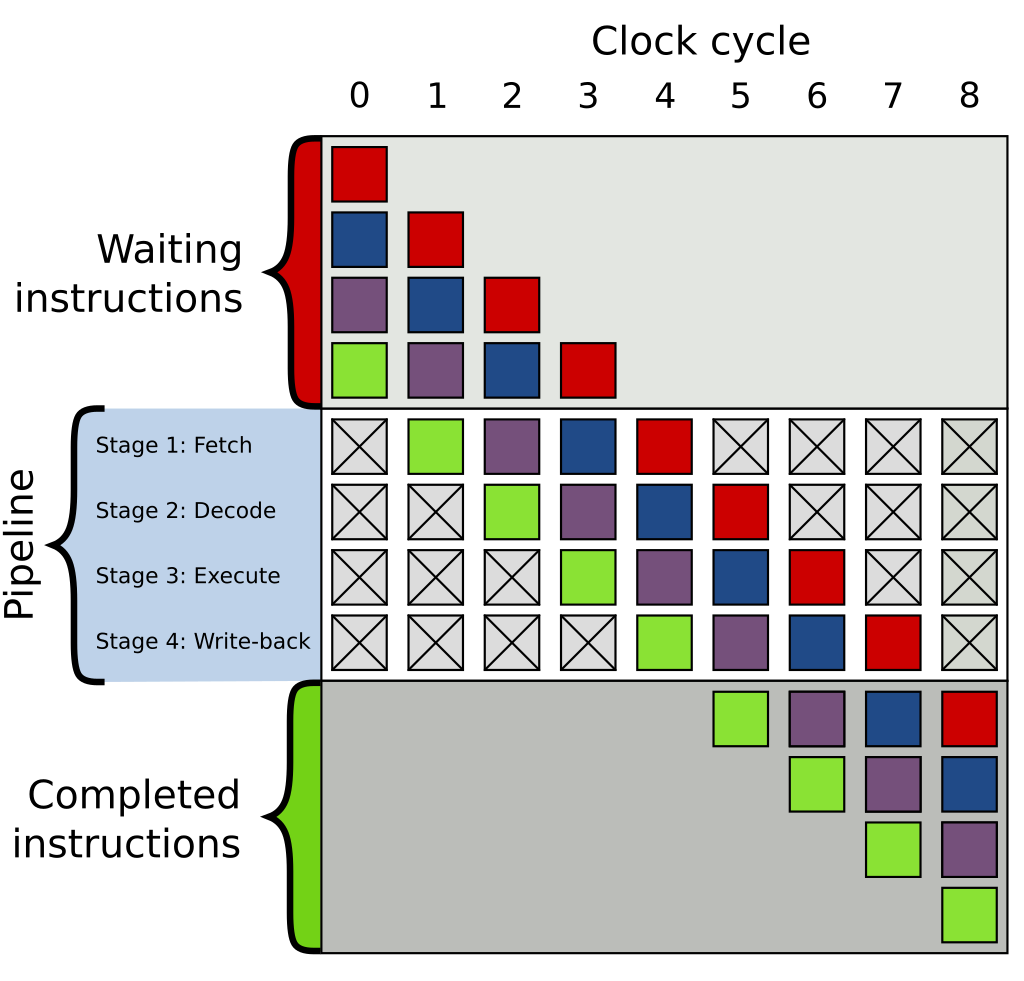
\includegraphics[width=0.3\textwidth]{imgs/pipeline.png}
    \caption{Prozessor Pipeline~\cite{wikipedia_pipeline}}\label{fig:pipeline}
\end{figure}

Datenparallelität beschreibt die Aufteilung der Daten in mehrere Teile, die mit mehreren Bearbeitungseinheiten parallel verarbeitet werden. Die Daten müssen dafür unabhängig von einander sein.
Beide Ansätze können die Performance von Algorithmen verbessern, und können auch kombiniert werden um die Vorteile beider Ansätze zu nutzen. Um beide Ansätze zu kombinieren, könnten mehrere Pipelines entworfen werden,
die jeweils verschidene Daten bearbeiten.



\subsection{Partial Reconfiguration}
Partial Reconfiguration (PR) ist ein Konzept, welches aktuelle FPGAs unterstützen. PR bietet die Möglichkeit, Teile des FPGAs zur Laufzeit zu verändern,
ohne das gesamte FPGA neu zu konfigurieren oder das FPGA offline nehmen zu müssen. Dies ermöglicht es, verschiedene Funktionen auf einem FPGA zu implementieren
und bei Bedarf zu wechseln. Umkonfiguration während der Laufzeit bietet offensichtlich Pozenzial für Beschleunigung, da mehr Algorithmen implementiert
werden können, als gleichzeitig auf dem FPGA Platz haben. Eine Problematik ist jedoch, dass die Umkonfiguration Zeit in Größenordnung von Millisekunden benötigt.
Zudem ist die PR-Region nicht dynamisch anpassbar, wodurch bei der Umkonfiguration zu anderen Algorithmen Ressourcen auf dem FPGA verschwendet werden, wenn der
Ressourcenaufwand der neuen Algorithmen geringer ist.

Das Projekt DoppioDB~\cite{istvan_glass_2019} nutzt PR, um verschiedene Algorithmen auf einem FPGA zu implementieren und bei Bedarf zu wechseln.




\subsection{BitWeaving}
BitWeaving ist ein Algorithmus, der in~\cite{li_bitweaving_2013} vorgestellt wird. Der Algorithmus stellt eine Methode dar, Spaltenscanoperationen durchzuführen, indem
die Daten mehrerer Zeilen als Bitvektor codiert in einem Prozessorwort gespeichert und verarbeitet werden. Zwei Varianten des Algorithmus werden vorgestellt, BitWeaving H und BitWeaving V,
die sich in der Art und Weise unterscheiden, wie die Daten in den Prozessorworten gespeichert werden. BitWeaving H speichert die Daten zeilenweise in den Prozessorworten, was bedeutet, dass
Daten in einem Prozessorwort und nicht über mehrere Prozessorworte hinweg gespeichert werden. BitWeaving V speichert die hingegen Daten spaltenweise in den Prozessorworten. BitWeaving H ist
der betrachtete Algorithmus in~\cite{lisa_column_2018}.

BitWeaving stellt ein arithmetisches Framework dar, mit welchem es möglich ist über mehrere Schritte und Bitmasken mit Daten gefüllte Prozessorworte mit einem Prädikatsvektor zu vergleichen.
Die Leistung von BitWeaving ist, dass die benötigten Taktzyklen für die Verarbeitung von einer Zeile stark reduziert wird, da in jedem Takt mehrere Zeilen pro Prozessorwort verarbeitet werden können~\cite{li_bitweaving_2013}.
Die amortisierte Taktzyklenzahl pro Zeile wird durch BitWeaving zum Teil auf unter 1 reduziert, im Vergleich zu vielen Taktzyklen pro Zeile bei herkömmlichen Methoden~\cite{li_bitweaving_2013}.



\section{Einordnung der Situation} \label{sec:einordnung}
Die Rolle von FPGAs in Datenbanksystemen ist laut~\cite{istvan_glass_2019} aktuell einem Wandel unterzogen. Während bei FPGAs in der Vergangenheit
Herausforderungen die Potenziale überwogen haben, bieten aktuelle Entwicklungen neue Möglichkeiten für den Einsatz von FPGAs in Datenbanksystemen.

~\cite{istvan_glass_2019} stellt diese Entwicklung als Gegensätze von Pessimismus der Vergangenheit und Optimismus der Gegenwart und Zukunft dar.

\subsection{Pessimismus}
Der Pessimismus der Vergangenheit begründete sich fundamental in drei Problemen.

Erstens war die Anbindung der On-the-Side Beschleuniger an die CPU ein Flaschenhals, da die Kommunikation in beiden Richtungen über
einen Bus erfoglen musste, welcher zu hohe Latenzen bot.~\cite{istvan_glass_2019} On-the-Side Beschleuniger waren
die gängige Architektur, um Datenbankoperationen zu beschleunigen, welche nicht im Datenpfad durchgeführt werden können.
Koprozessor Architekturen wurden von Chipherstellern nicht wirklich angeboten und waren somit nicht weit verbreitet.

Zweitens profitieren nicht alle Algorithmen von der Beschleunigung durch FPGAs. Iterative Algorithmen, die auf den Ergebnissen vorheriger
Iterationen aufbauen, können nicht von der hohen Parallelität von FPGAs profitieren. CPUs sind in diesen Fällen performanter,
da die hohen Taktraten die itertiven Instruktionen abarbeiten können. Auch weit verzweigte Algorithmen, mit vielen If-Else Anweisungen
sind nicht für FPGAs geeignet, da jeder Pfad im FPGA implementiert werden muss, was zu hohen Ressourcenverbrauch führt. Hoher Ressourcenverbrauch
wiederrum führt zu geringerer Parallelität, da weniger paralelle Pipelines implementiert werden können. Die Inkompatibilität von Algorithmen
wird durch den ersten Punkt noch verstärkt, da die schwierige Kommunikation zwischen CPU und FPGA die Entwickler dazu zwingt, gesamte Algorithmen
auf dem FPGA zu implementieren, anstatt nur die Teile, die von der Beschleunigung profitieren, um die Kommunikation zu minimieren~\cite{istvan_glass_2019}.

Drittens ist die direkte Konkurrenz von CPUs ein Hinderniss. CPUs sind sehr flexible, sie können theoretisch jeden Algorithmus
ausführen. Hinzu kommt, dass die Leistung der CPUs stetig steigt (Moores's Law) und die Taktraten immer höher werden. Durch den hohe
Zeit- und Ressourcenaufwand, welcher die Entwicklung von FPGA Beschleunigern mit sich bringt, war es häufig nicht praktikabel, FPGAs
anstelle von CPUs für Datenbankbeschleunigung zu nutzen.

\subsection{Optimismus}
Der Optimismus für die Gegenwart und Zukunft, den der Autor motiviert, basiert auf drei wesentlichen Entwicklungen.

Erstens haben sich die Architekturen verändert. Moderne FPGAs sind häufig als Koprozessoren direkt auf dem gleichen Chip wie die CPU integriert,
was die Latenzen und Bandbreitenprobleme der On-the-Side Beschleuniger, durch direkten Speicherzugriff des FPGAs, löst.
Diese enge Integration ermöglicht granulare Beschleunigung, bei der nur die Teile des Algorithmus, die von der Beschleunigung profitieren,
auf dem FPGA implementiert werden. Die erhöhte Verfügbarkeit von Koprozessor Architekturen bestärkt nun auch die Erforschung und Entwicklung
von FPGA Beschleunigern was zu einer Vielzahl von neuen Anwendungen führt~\cite{lisa_column_2018}~\cite{sidler_accelerating_2017}.

Ein anschauliches Beispiel ist die Nutzung von FPGAs in Cloud-Umgebungen. Große Anbieter wie Amazon, Baidu und Huawei bieten FPGAs stundenweise an,
damit Nutzer individuelle Beschleuniger implementieren können. Microsoft nutzt im Rahmen des Projekts Catapult FPGAs in der Azure-Cloud, um sowohl ihre
Infrastruktur als auch maschinelle Lernpipelines zu beschleunigen. Intel experimentiert zudem mit der Integration programmierbarer Elemente direkt in
ihre Xeon-CPUs, wodurch spezifische Benutzeranwendungen beschleunigt werden können~\cite{istvan_glass_2019}.


Zweitens haben sich die Workloads verändert. In der Vergangenheit wurden hauptsächlich klassische SQL-Operatoren
in Datenbank durchgeführt, welche auf der verfügbaren Hardware häufig Memory-bound waren, also durch die
Geschwindigkeit der Datentransfers limitiert. Durch neue Anwendungen wie Maschinelles Lernen und Künstliche Intelligenz
sind neue Workloads entstanden, die häufig Compute-bound sind, also durch die Geschwindigkeit der Berechnungen limitiert. Da diese Anwendungen viele Daten benötigen,
liegt es nahe, die Anwendungen als neue Datenbank Operatoren einzuführen. Für Compute-bound Workloads werden FPGAs wieder interessant, da sie durch ihre
hohe Parallelität und Rekonfigurierbarkeit die Berechnungen beschleunigen können.
Auch die Optimierung- und Entscheidungsprozesse innerhalb der Datenbanksysteme könnten durch Maschinelle Lernverfahren verbessert oder abgelöst werden, was ebenfalls
Potenziale für FPGAs bietet~\cite{istvan_glass_2019}.

Drittens ermöglichen hybride Ansätze eine bessere Nutzung der Stärken von FPGAs und CPUs. Durch die Kombination beider Technologien
können Algorithmen so aufgeteilt werden, dass die parallelisierbaren Teile auf dem FPGA und die sequentiellen Teile auf der CPU ausgeführt werden. Ein Beispiel dafür ist das
REGEXP\_LIKE Projekt~\cite{sidler_accelerating_2017}.


\section{BitWeaving Spalten Scan Beschleunigung} \label{sec:col_scan_acc}
Im Kontext veränderter Architekturen ordnet sich auch die Column Scan Acceleration~\cite{lisa_column_2018} ein. Dort wurde auf einem FPGA ein Beschleuniger implementiert, der
den BitWeaving H Algorithmus für einen Spaltenscan verwendet. Es wurden verschidenen Hardwareansätze verglichen und bewertet, um die beste Performance zu erzielen.

\subsection{Architektur}
Die Forschung von~\cite{lisa_column_2018} baut auf der Zynq Ultrascale+ Architektur von Xilinx auf. Die Plattform ist zweiteilig aus Steuersystem mit
vier ARM Cortex-A53 Kernen mit 1.2GHz Takt und 4GB DDR4 Speicher und Logikbereich mit FPGA und 512MB DDR4 Speicher aufgebaut~\cite{lisa_column_2018}.
Durch 32-bit -- 128-bit Busse kann der Logikbereich auf den Speicher des Steuersystems zugreifen. Diese Busse werden `direct memory access' (DMA) genannt.
Die Architektur ist klar als Koprozessor Architektur einzuordnen, da der FPGA direkt auf dem gleichen Chip wie die CPU sitzt und direkten Speicherzugriff hat.


\subsection{Grundlegendes Vorgehen}
Die Basis der Implementierung bildet eine Pipeline, die die Daten in mehreren Schritten verarbeitet und die durch den BitWeaving Algorithmus motiviert ist. Die Pipeline besteht aus Leseblöcken,
Verarbeitungsblöcken und Schreibeblöcken. Die Leseblöcke bekommen sowohl die zu evaluierenden Daten als auch den Prädikatsvektor von einem DMA\@.
Der Prädikatsvektor wird nur zu Begin geladen, da sich dieser nicht verändert.
Verarbeitugsblöcke führen die eigentliche BitWeaving Operation durch und von ihnen gibt es so viele Blöcke wie benötigt werden um die Schritte des Algorithmus durchzuführen.
Der BitWeaving Gleichheitscheck benötigt beispielsweise 4 Blöcke um die Masken und Verknüpfungen durchzuführen. Die Schreibeblöcke schreiben die Ergebnisse zurück in den
Speicher des Steuersystems. Alle Blöcke werden pipelinetypisch hintereinander geschaltet, sodass die Daten durch die Pipeline fließen und die Ausgaben des vorherigen
Blocks die Eingaben des nächsten Blocks sind~\cite{lisa_column_2018}.

Um die verschidene Ansätze zu vergleichen, wurde ein Datensatz aus 1 Million Zeilen verwendet. Pro Prozessorwort wurden 16 Zeilen repräsentiert. Verglichen wurden in dieser ersten Auswertung
die BitWeaving Implementierung auf den ARM Kernen des Steuersystems mit ein bis vier Kernen (in Abbildung~\ref{fig:eval}: `X Cores') und die BitWeaving Implementierung
auf dem FPGA mit verschiedenen DMA Busbreiten von 32-bit, 64-bit und 128-bit (in Abbildung~\ref{fig:eval}: `BASIC X', nach der Breite der verarbeiteten Daten) 1 ARM Kern
erreichte einen Durchsatz von 1.9 GB/s, 4 Kerne ca. 4.8 GB/s. Der FPGA erreichte mit 32-bit DMA 1.1GB/s, mit 64-bit DMA 1.9GB/s und mit 128-bit DMA 3.9GB/s.
Die erste Auswertung zeigt, dass der Entwurf mit 128-bit DMA die beste Performance erzielt, da dieser die meisten Daten gleichzeitig verarbeiten kann,
aber immernoch schlechter abschneidet als vier ARM Kerne~\cite{lisa_column_2018}.


\subsection{Verschiedene Entwürfe}

Um die Parallelität und damit auch den Durchsatz des Systems zu erhöhen, wurde Datenparallel gearbeitet, indem mehrere Pipelines implementiert wurden. Es werden
also beide Arten der Parallelität aus~\cite{istvan_glass_2019} aufgegriffen. Jede Pipeline
hat einen eigenen DMA und kann so unabhängig von den anderen Pipelines Daten aus dem Speicher laden. Da bei einem Spaltenscan die Daten unabhängig von einander sind,
können so viele Zeilen gleichzeitig evaluiert werden.

Den Ergebnissen aus der ersten Auswertung folgend wurde mit 128-bit DMA gearbeitet, da dieser die beste Performance erzielt hat. Des weiteren wurde einen neue Pipeline Stufe
hinzugefügt, welche mehrere Datenworte zu einem längeren Datenwort kombiniert. Diese Combiner-Stufe führt die Pipelines direkt nach den DMA Blöcken zusammen. Die Verarbeitungsblöcke
müssen jetzt mit längeren Datenwörtern arbeiten, 256-bit bei zwei DMAs 384-bit bei drei DMAs und 512-bit bei vier DMAs. Durch die erhöhte Menge an gleichzeitig verarbeiteten Daten
wurde ein erhöhter Durchsatz erwartet und auch gemessen (In Abbildung~\ref{fig:eval}: `COMBINED X'). Mit zwei DMAs wurde ein Durchsatz von 7.7 GB/s erreicht, mit drei DMAs 7.5GB/s
und mit vier DMAs 6.5GB/s.
Zwei DMAs bieten den höchsten Durchsatz, da die DMAs durch die Combiner-Stufe voneinander abhängen, und so gewartet werden muss, bis alle DMAs vom DDR4 Kontroller bedient wurden.
Außerdem takten die Entwürfe mit mehr als zwei DMAs nur mit 200MHz, während die Entwürfe mit zwei 250MHz takten, da die Combiner-Stufe die Taktfrequenz, aufgrund der großen
Datenworte, reduziert.

Durch diese Erkenntnis wurde ein weiterer Ansatz (In Abbildung~\ref{fig:eval}: `INDEP X') eingeführt, bei welchem die Pipelines bis zum Ende getrennt voneinander sind und
somit keine Abhängigkeiten zwischen den DMAs bestehen. Der Combiner fällt weg, dafür werden nun 4 parallele Verarbeitungsblöcke benötigt, welche auf 128-bit Worten
arbeiten. Es können auf diese Weise neue Höchstewerte im Durchsatz erzielt werden,
7.8GB/s mit zwei DMAs, 8.9GB/s mit drei DMAs und 8.1GB/s mit vier DMAs. Vier DMAs reduzieren den absoluten Durchsatz, da der DDR4 Kontroller
nicht genug Bandbreite für vier DMAs bieten kann und der
vierte DMA nicht direkt an den DDR4 Kontroller angeschlossen ist.

Durch die Erkenntnis aus dem COMBINED Ansatz, dass Verarbeitugsblöcke mit 256-bit gute Performance bieten kann, und die Erkenntnis aus dem INDEP Ansatz, dass
unabhängige Pipelines den Durchsatz erhöhen, wurde ein neuer Ansatz (In Abbildung~\ref{fig:eval}: `HYBRID X') entwickelt, welcher beide Ansätze kombiniert.
Jede Pipeline ist von Anfang bis Ende unabhängig, verfügt aber trotzdem über ein 128-bit zu 256-bit Combiner. Der Combiner kombiniert jeden zweiten Takt zwei 128-bit Worte
vom gleichen DMA zu einem 256-bit Wort. Dadurch können die Verarbeitungsblöcke auf 256-bit Worten arbeiten. Es entstehen so Entwürfe mit zwei DMAs, welche 512-bit Daten verarbeiten
(Hybrid 512), mit drei DMAs, welche 768-bit Daten verarbeiten (Hybrid 768) und mit vier DMAs, welche 1024-bit Daten verarbeiten (Hybrid 1024). Zwei DMAs erreichen 7.7GB/s, drei DMAs 9.2GB/s
und vier DMAs 8.4GB/s. Drei DMAs erzielen erneut das beste Ergebnis.


Der letzte Entwurf in~\cite{lisa_column_2018} adressiert die Einschränkungen durch Speicherbandbreite, indem mehrere Speicher gleichzeitig genutzt werden
(in Abbildung~\ref{fig:eval}: `HYBRID2 X').
Im untersuchten hybriden System gibt es zwei DDR4-Speicher: einen im Steuersystem (PS) und einen im Logikbereich (PL). Durch Hinzufügen eines zusätzlichen DMA-Controllers
und einer FIFO-Stufe zwischen Combiner und Verarbeitungseinheit konnten Designs mit bis zu fünf DMAs und einer kombinierten Datenbreite von 1280 Bits realisiert werden.
Die Daten wurden hierfür auf die DDR4 Speicher nach Anzahl der angeschlossenen DMAs aufgeteilt.

Die Ergebnisse zeigen, dass durch die Verwendung von PL- und PS-Speicher gleichzeitig der Durchsatz auf 12 GB/s erhöht werden konnte. Dabei bleibt jedoch die Herausforderung bestehen,
dass nicht alle vier PS-DMA-Kanäle vollständig ausgelastet werden können, wodurch der optimale Ansatz bei drei PS-DMA-Kanälen und einem PL-DMA-Kanal liegt.

\subsection{Vergleich der Entwürfe}

Die Analyse der verschiedenen Ansätze zeigt, dass die Unabhängigkeit zwischen Pipelines entscheidend für die Performance ist. Designs,
die auf kombinierter Verarbeitung basieren, sind bei geringen Datenbreiten effizient, während unabhängige Verarbeitungsansätze für
höhere Datenbreiten besser geeignet sind. Hybride Ansätze, die beide Optimierungsstrategien kombinieren, bieten die höchste Leistung,
verwenden jedoch mehr Ressourcen~\cite{lisa_column_2018}.

\subsection{Zusammenfassung der Erkenntnisse}

Die vorgestellten Optimierungen zeigen die Potenziale von FPGA-unterstützten Spaltenscans auf. Abhängig von der verwendeten Architektur kann
der Durchsatz signifikant gesteigert werden, insbesondere durch eine geschickte Kombination aus paralleler Verarbeitung und der Nutzung mehrerer
Speicher. Die besten Resultate wurden durch das HYBRID2 1024 Design mit einer Durchsatzrate von 12 GB/s erzielt (siehe Abbildung~\ref{fig:eval}). Zukünftige Arbeiten
könnten sich darauf konzentrieren, die Designs weiter an unterschiedliche FPGA- und Speicherarchitekturen anzupassen~\cite{lisa_column_2018}.


\begin{figure}[htbp]

    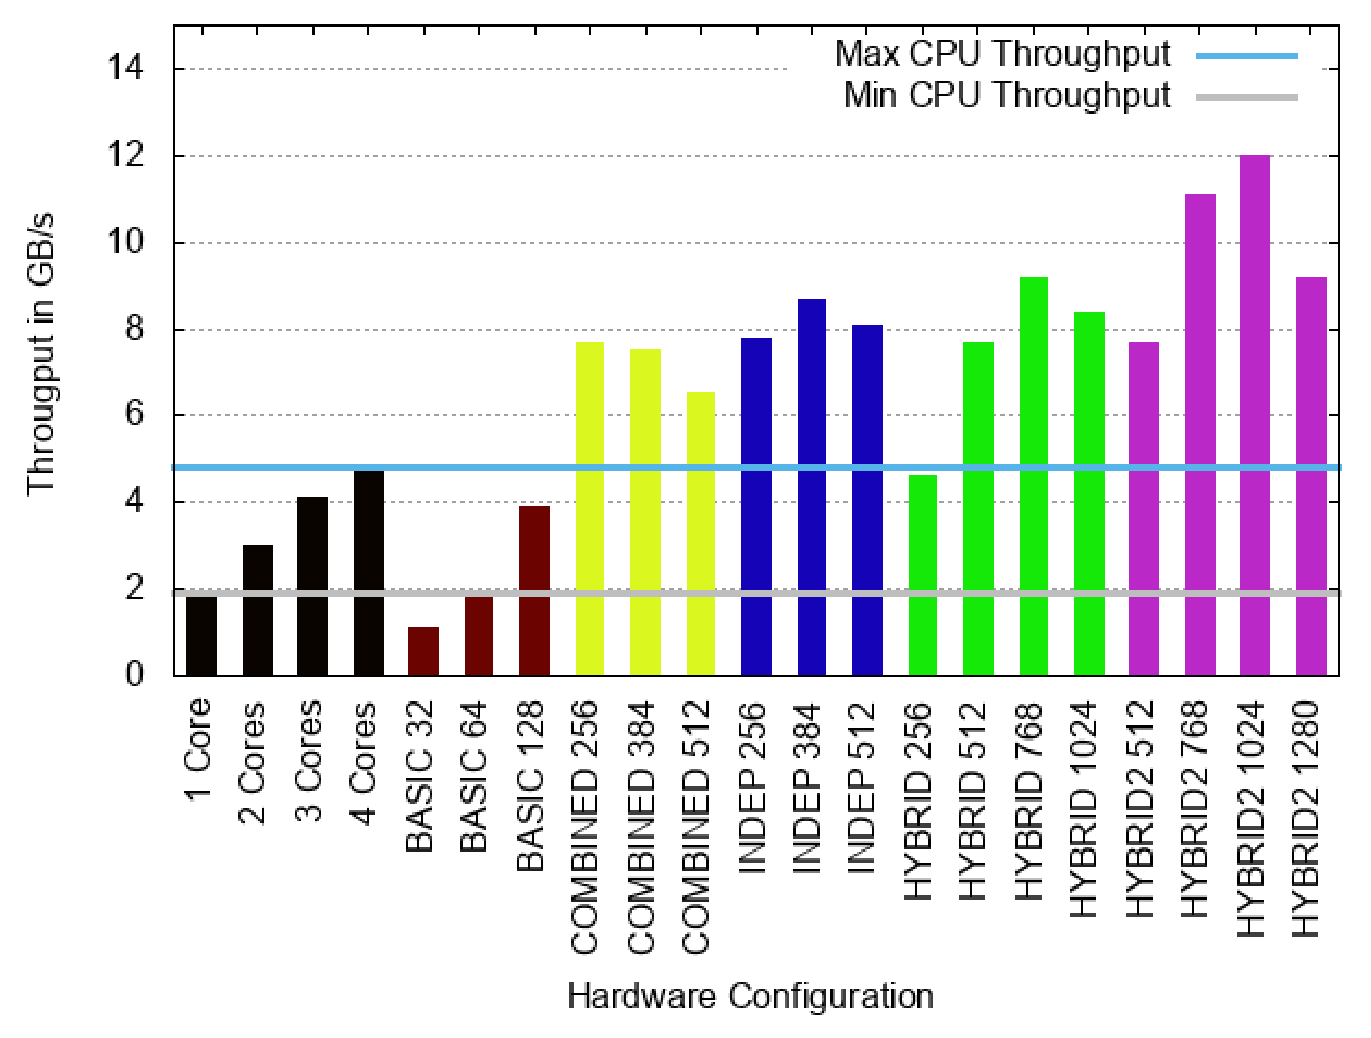
\includegraphics[width=0.47\textwidth]{imgs/eval.png}
    \caption{Ergebnisse der Evaluation~\cite{lisa_column_2018}}
    \label{fig:eval}
\end{figure}


\section{Andere Ansätze} \label{sec:andere_ansätze}
Auch Zsolt Istv\'{a}n stellt Ansätze vor, die sich mit In-Data-Path Beschleunigern, hybriden Ansätzen und intelligenten Speichersystemen beschäftigen. Diese Ansätze
zeigen Beispiele auf, wie FPGAs in Datenbanksystemen eingesetzt werden können und wie die beschriebenen Herausforderungen überwunden werden können~\cite{istvan_glass_2019}.

\subsection{IBEX}
IBEX ist ein FPGA-basierter Beschleuniger für Datenbanken, der in~\cite{istvan_glass_2019} vorgestellt wird. IBEX ist ein In-Data-Path Beschleuniger,
ist also zwischen SSD und der CPU platziert. Die Daten werden mit gleicher Bandbreite verarbeitet, wie sie von der SSD
ankommen. Der FPGA führt SQL-Operatoren aus, welche die Datenmenge reduzieren, also beispielsweise Filter und Aggregationen, nicht aber Operatoren,
die die Datenmenge erhöhen können, wie Joins. IBEX verwendet auch einen hybriden Ansatz, um Aggregate zu berechnen. Die Aggregatfunktionen werden auf dem FPGA
mit einem Hashtable berechnet, welcher mit fester Größe im RAM verortet ist. Dies ermöglicht gleiche Laufzeiten, unabhängig von den Daten, da der Hashtable nicht
dynamisch vergrößert werden muss, wodurch aber die Anazhl der Gruppen bei Aggregatbildung limitiert ist. Um dieses Limit zu umgehen, gibt der FPGA Teilaggregate
weiter, sobald der Hashtable keinen Platz mehr für neue Gruppen hat. Die CPU vereinigt dann die Teilaggregate zu einem Endergebnis auf eine Weise, das die Bearbeitung
von der Arbeit des FPGAs in jedem Fall profitiert. Der FPGA kann so die Datenmenge reduzieren und die CPU kann die reduzierte Datenmenge effizienter verarbeiten.

\subsection{Caribou}
Caribou ist ein intelligentes, verteiltes Speichersystem, das speziell für effiziente Datenverarbeitung und -speicherung in modernen Rechenzentren entwickelt wurde.
Durch die Integration von Near-Data-Processing wird ein Großteil der Berechnungen direkt an den Speicherknoten durchgeführt, wodurch die Bewegung großer Datenmengen
über das Netzwerk minimiert wird. Das System ist auf FPGAs aufgebaut, um eine parallele Verarbeitung und geringe
Latenzzeiten sowie eine hohe Durchsatzrate gewährleisten.

Das System nutzt ein einfaches Key-Value-Interface, das über TCP/IP zugänglich ist, und bietet gleichzeitig eine Replikation der Daten, um Fehlertoleranz
und Konsistenz sicherzustellen. Caribou ist somit laut~\cite{istvan_caribou_2017}
eine leistungsstarke, energieeffiziente Lösung für datenintensive Anwendungen in verteilten Systemen.

\subsection{DoppioDB}
Das Projekt DoppioDB zeigt einen Ansatz, indem die Datenbank die FPGA-Steuerung
übernimmt und Slots auf dem FPGA verwendet, welche vom Betriebssystem aufgesetzt wurden.
Die Slots werden Hardware-Threads gegannt, da sie wie Software-Threads angesprochen werden und durch Partial Rekonfiguration von der Datenbank auf die benötigten Aufgaben
angepasst werden. Dabei wurde über SQL hinausgehend Funktionalität für maschinelles Lernen integriert, wie z. B.
stochastische Gradientenabstiege und Entscheidungsbaum-Inferenz~\cite{istvan_glass_2019}.



\subsection{REGEXP\_LIKE}
Ein vorgestelltes Projekt befasst sich mit der Optimierung des REGEX\_LIKE Operators, welcher reguläre Ausdrücke auf Datenbanken anwendet~\cite{istvan_glass_2019}. So können beispielsweise
alle Zeilen einer Tabelle selektiert werden, die in einer Spalte einen bestimmten regulären Ausdruck erfüllen. Der Operator wurde auf einem FPGA implementiert
und zeigt die Nutzung von hybriden Ansätzen, indem die relevanten Daten so weit wie möglich auf dem FPGA verarbeitet werden und nur falls nötig auf der CPU
nachbearbeitet werden~\cite{sidler_accelerating_2017}. So können alle REGEXP\_LIKE-Anfragen durch die Beschleunigung profitieren, da nicht vollständig passende
reguläre Ausdrücke nicht abgewiesen und damit vollständig auf der CPU verarbeitet werden müssen.

Der Reguläre Ausdruck wird an an einer Wildcard-Position aufgeteil, so dass zwei unabhängige reguläre Ausdrücke entstehen. Der FPGA gibt dann, zusammen mit einem Index
alle Zeilen zurück, die den ersten regulären Audruck erfüllen. Die CPU überprüft dann, ob die Zeilen vom Index aus auch den zweiten regulären Ausdruck erfüllen.
Der verwendete Ausdruck in ist in Listing~\ref{lst:regexp} zu sehen. Der FPGA bearbeitet den Ausdruck bis zur zweiten
Wildcard und die CPU muss dann nur noch nach `delivery' suchen. Sidler et al. zeigen, dass der REGEXP\_LIKE Operator auf einem FPGA um den Faktor 13 beschleunigt wird,
wenn die CPU kein Nachbearbeitung machen muss, und selbst wenn die CPU jeden Datenpunkt nachbearbeiten muss, wird die Bearbeitung immernoch beschleunigt~\cite{sidler_accelerating_2017}.


\begin{lstlisting}[language=SQL,frame=single,caption={Regulärer Ausdruck aus \cite{sidler_accelerating_2017}},label={lst:regexp}, float=b]
SELECT count(*)
FROM address_tables
WHERE REGEXP_LIKE(address_string,
'(Strasse|Str\.).*(8[0-9]{4}).*delivery');
\end{lstlisting}

\section{The Road that lies ahead} \label{sec:road_ahead}
Ein zentraler Aspekt der zukünftigen Datenbankentwicklung ist die Integration programmierbarer Hardware wie FPGAs, die zwar neu konfigurierbar, jedoch nicht so flexibel wie Software sind~\cite{istvan_glass_2019}.
Die Kernfrage hierbei ist laut Zsolt Istv\'{a}n wer die Kontrolle über die Beschleunigungsfunktionen übernimmt --- das Betriebssystem oder die Datenbank selbst.




\subsection{Betriebssystem- oder Datenbankverwaltung?}

Wenn das Betriebssystem die Kontrolle behält, muss die Datenbank Strategien entwickeln, um von hardwarebasierten Beschleunigungsmöglichkeiten zu profitieren,
die vom Infrastruktur- oder Cloudanbieter bereitgestellt werden. Hierbei könnten bereits etablierte Techniken zur Code-Optimierung für spezifische CPU Features,
wie SIMD-Einheiten, als Grundlage dienen~\cite{istvan_glass_2019}.

Übernimmt hingegen die Datenbank die Kontrolle, eröffnen sich größere Gestaltungsspielräume. Die Datenbank könnte benutzerdefinierte Hardware-Beschleuniger entwickeln,
die exakt auf ihre Bedürfnisse abgestimmt sind, und diese sogar zur Laufzeit synthetisieren (siehe DoppioDB).
Offen ist hierbei, wie eine Bibliothek von Hardwareentwürfen aussehen könnte, die von Datenbanken sinnvoll und wiederholt eingesetzt werden können~\cite{istvan_glass_2019}.


\subsection{Weitere Herausforderungen}
Neben der Art der Hardwareentwürfe ist auch der breite Einsatz derselben problematisch, da FPGAs, im Gegensatz zu CPUs oder GPUs keine feste Architektur haben
und Datenbanksysteme daher nur schwierig für FPGAs optimieren können. Compilier Ideen könnten helfen, von der heterogenen Hardware zu abstrahieren und so
die Entwicklung von FPGA-Beschleunigern zu vereinfachen~\cite{istvan_glass_2019}.

Das Ressourcenproblem wird auch nocheinmal thematisiert, also die Begrenztheit der
Ressourcen auf einem FPGA, die es unmöglich machen alle Algorithmen auf einem FPGA zu implementieren. Es wird auf hybride Ansätze verwiesen (siehe oben)~\cite{istvan_glass_2019}.

\section{Fazit} \label{sec:fazit}
Die Nutzung von FPGAs in Datenbanksystemen bietet vielversprechende Möglichkeiten zur Beschleunigung von Datenbankoperationen. Durch die hohe Parallelität
und Flexibilität von FPGAs können spezifische Algorithmen effizienter ausgeführt werden als auf herkömmlichen CPUs. Verschiedene Ansätze wie IBEX, Caribou,
DoppioDB und REGEXP\_LIKE zeigen, dass FPGAs sowohl als In-Data-Path Beschleuniger als auch als Koprozessoren eingesetzt werden können.
Die Nutzung des BitWeaving Algorithmus~\cite{lisa_column_2018} zeigt, dass auch Optimierungen aus anderen Hardwarebereichen auf FPGAs verwendet
werden können und dass die Optimierung von Hardwareentwürfen die Performance von FPGA-Beschleunigern signifikant verbessern kann.
Die Herausforderungen, wie die begrenzten Ressourcen und die Komplexität der Entwicklung, können durch hybride Ansätze und die Integration von FPGAs in moderne
Architekturen überwunden werden.
Besonders der Wandel der angebotenen Architekturen, wie die Integration von FPGAs in Cloud-Umgebungen, stimmt optimistisch für die Zukunft von FPGAs in Datenbanksystemen
und die Forschung und Entwicklung derselben.
Die Zukunft der Datenbankbeschleunigung wird maßgeblich davon abhängen, wie gut es gelingt, die Vorteile von FPGAs in die
bestehenden Systeme zu integrieren und die Entwicklung von FPGA-Beschleunigern zu vereinfachen.

\bibliographystyle{IEEEtran}
\bibliography{FPGAs}

\end{document}
